\documentclass[a4paper, 12pt]{report}

%%%%%%%%%%%%
% Packages %
%%%%%%%%%%%%

\usepackage[english]{babel}
\usepackage[noheader]{packages/sleek}
\usepackage{packages/sleek-title}
\usepackage{packages/sleek-theorems}
\usepackage{packages/sleek-listings}

\usepackage{import}

\usepackage{fontspec}
\usepackage[CheckSingle, CJKmath]{xeCJK}
\usepackage{CJKulem}

\setCJKmainfont{Times New Roman}

\usepackage{packages/rish}

%%%%%%%%%%%%%%
% Title-page %
%%%%%%%%%%%%%%

\logo{./resources/pdf/blank.png}
\institute{輔仁大學資訊工程學系}
\faculty{畢業專題報告}
\department{B03 組}
\title{Rish Engine - 2D 遊戲引擎}
\subtitle{從零開始自幹遊戲引擎}
\author{\textit{成員} \\
	406262515 \textsc{鍾秉桓} me@roy4801.tw\ \ \ \ \ \ \ \ \ \ \ \ \ \ \\
    406262084 \textsc{梁博全} me@icejj.tw\ \ \ \ \ \ \ \ \ \ \ \ \ \ \ \ \ \ \  \\
    406262319 \textsc{黃育晧} suntalk1224@gmail.com\ \  \\
    406262163 \textsc{黃品翰} william31212@gmail.com \\
    \ \\
    報告編號: CS109-PR-B03 \\
    \ \\
    \textit{指導教授} \\
    鄭進和
}
%\supervisor{Linus \textsc{Torvalds}}
%\context{Well, I was bored...}
\date{\today}

%%%%%%%%%%%%%%%%
% Bibliography %
%%%%%%%%%%%%%%%%

\addbibresource{./resources/bib/references.bib}

%%%%%%%%%%
% Others %
%%%%%%%%%%

\lstdefinestyle{latex}{
    language=TeX,
    style=default,
    %%%%%
    commentstyle=\ForestGreen,
    keywordstyle=\TrueBlue,
    stringstyle=\VeronicaPurple,
    emphstyle=\TrueBlue,
    %%%%%
    emph={LaTeX, usepackage, textit, textbf, textsc}
}

\FrameTBStyle{latex}

\def\tbs{\textbackslash}

%%%%%%%%%%%%
% Document %
%%%%%%%%%%%%

\begin{document}
    % \maketitle
    \romantableofcontents

    \listoffigures

    % \chapter{摘要}

\section{背景簡介}

本專題是以 C++ 開發之 2D 遊戲引擎,開發者可以使用引擎提供之編輯器(RishEditor)編輯遊戲場景(Scene),並且可以對遊戲物件(Entity)附加遊戲邏輯(使用C++撰寫,並和編輯器一同編譯),
並支援 Batch Rendering \footnote{一種 Rendering 技巧,可支援同屏幕高達 100000 個 sprites} 、2D Lighting (Point Light, Ambient Light), Particle System, Constrain-based Physics (支援圓形、多邊形等)

\section{問題說明}

TODO

\section{實作結果}

TODO 本專題製作解決問題方法、創新所在、與實作結果等概要陳述

\newpage
    % \chapter{緒論}

\section{動機}

隨著遊戲的發展,現代的遊戲越來越趨於複雜,從數人的小型獨立製作,到數百人的大型 3A 級遊戲,遊戲的規模與以前不可同日而語,現今一個獨立開發工作室製作的 2D 遊戲,
在十多年前要達到同樣的規模可能要數十人的團隊才可能達到,而這些節省下來的時間成本,就是多虧了遊戲引擎的強大之處。現代遊戲引擎的複雜度,先進的圖學技術,複雜的物理模擬,
是需要一個具有規模的團隊來開發的,我們嘗試以此為目標,試著實作了一個具有一定規模的 2D 遊戲引擎。

\section{問題描述}

\subsection{歷史介紹}

最初並沒有所謂的遊戲引擎,遊戲常常是重頭開始建構(from scratch)的,這個概念被眾人所知最早是由 Jhon Carmack 發揚光大,他為 Doom 以及 Quake 系列遊戲開發的 3D 遊戲引擎,
深深地影響了遊戲業界,為早期(1990末)的遊戲業界標準,並促成引擎授權的商業模式,使得遊戲軟體的規模上升。

\subsection{遊戲是什麼}
電腦遊戲的技術本質是實時(real-time)可交互(interactive)的程式,遊戲程式會模擬出不精確但足以表現的遊戲世界,並且根據玩家的輸入做出相對的輸出(例如操作搖桿控制角色等),
通常遊戲會實作遊戲循環(Game Loop),更新遊戲邏輯、物理模擬、更新 AI 等。而通常遊戲要維持在每秒更新 60 幀才能保證流暢運行(低於 60 fps 通常會感覺卡頓),
也就是要在 16 毫秒內做完所有的遊戲更新並渲染到螢幕上頭,更何況在 VR 上要維持 90 FPS 才不會感覺暈眩,這也是為甚麼遊戲會如此要求效能。

\subsection{遊戲引擎是什麼}

遊戲引擎(Game Enigne)從字面上解釋是驅動遊戲的基礎程式,因此遊戲引擎須具備了窗口管理、輸出入管理、渲染(Rendering)系統、物理(Physics)系統…等子系統,除了基礎程式之外,
要是一個遊戲引擎還必須要有讓遊戲開發者使用之工具(可視化、非可視化),可能是單個工具或一整個工具鏈(Toolchain),使得遊戲開發者可以用該工具開發遊戲(Developing)、
進行測試(Debugging)、封裝發布(Shipping)等,否則就只能被稱為遊戲框架(Game Framework)。
遊戲引擎會讀入自訂的資源(Asset)格式 \footnote{常常是為了效能才會這樣做},並且有工具支援設計師將素材(貼圖、音效、模型等)轉換成引擎的格式,或是引擎工具可以直接產生,
因此遊戲引擎可以說是專門開發遊戲的開發環境。

\subsection{遊戲引擎具備的功能}

TODO

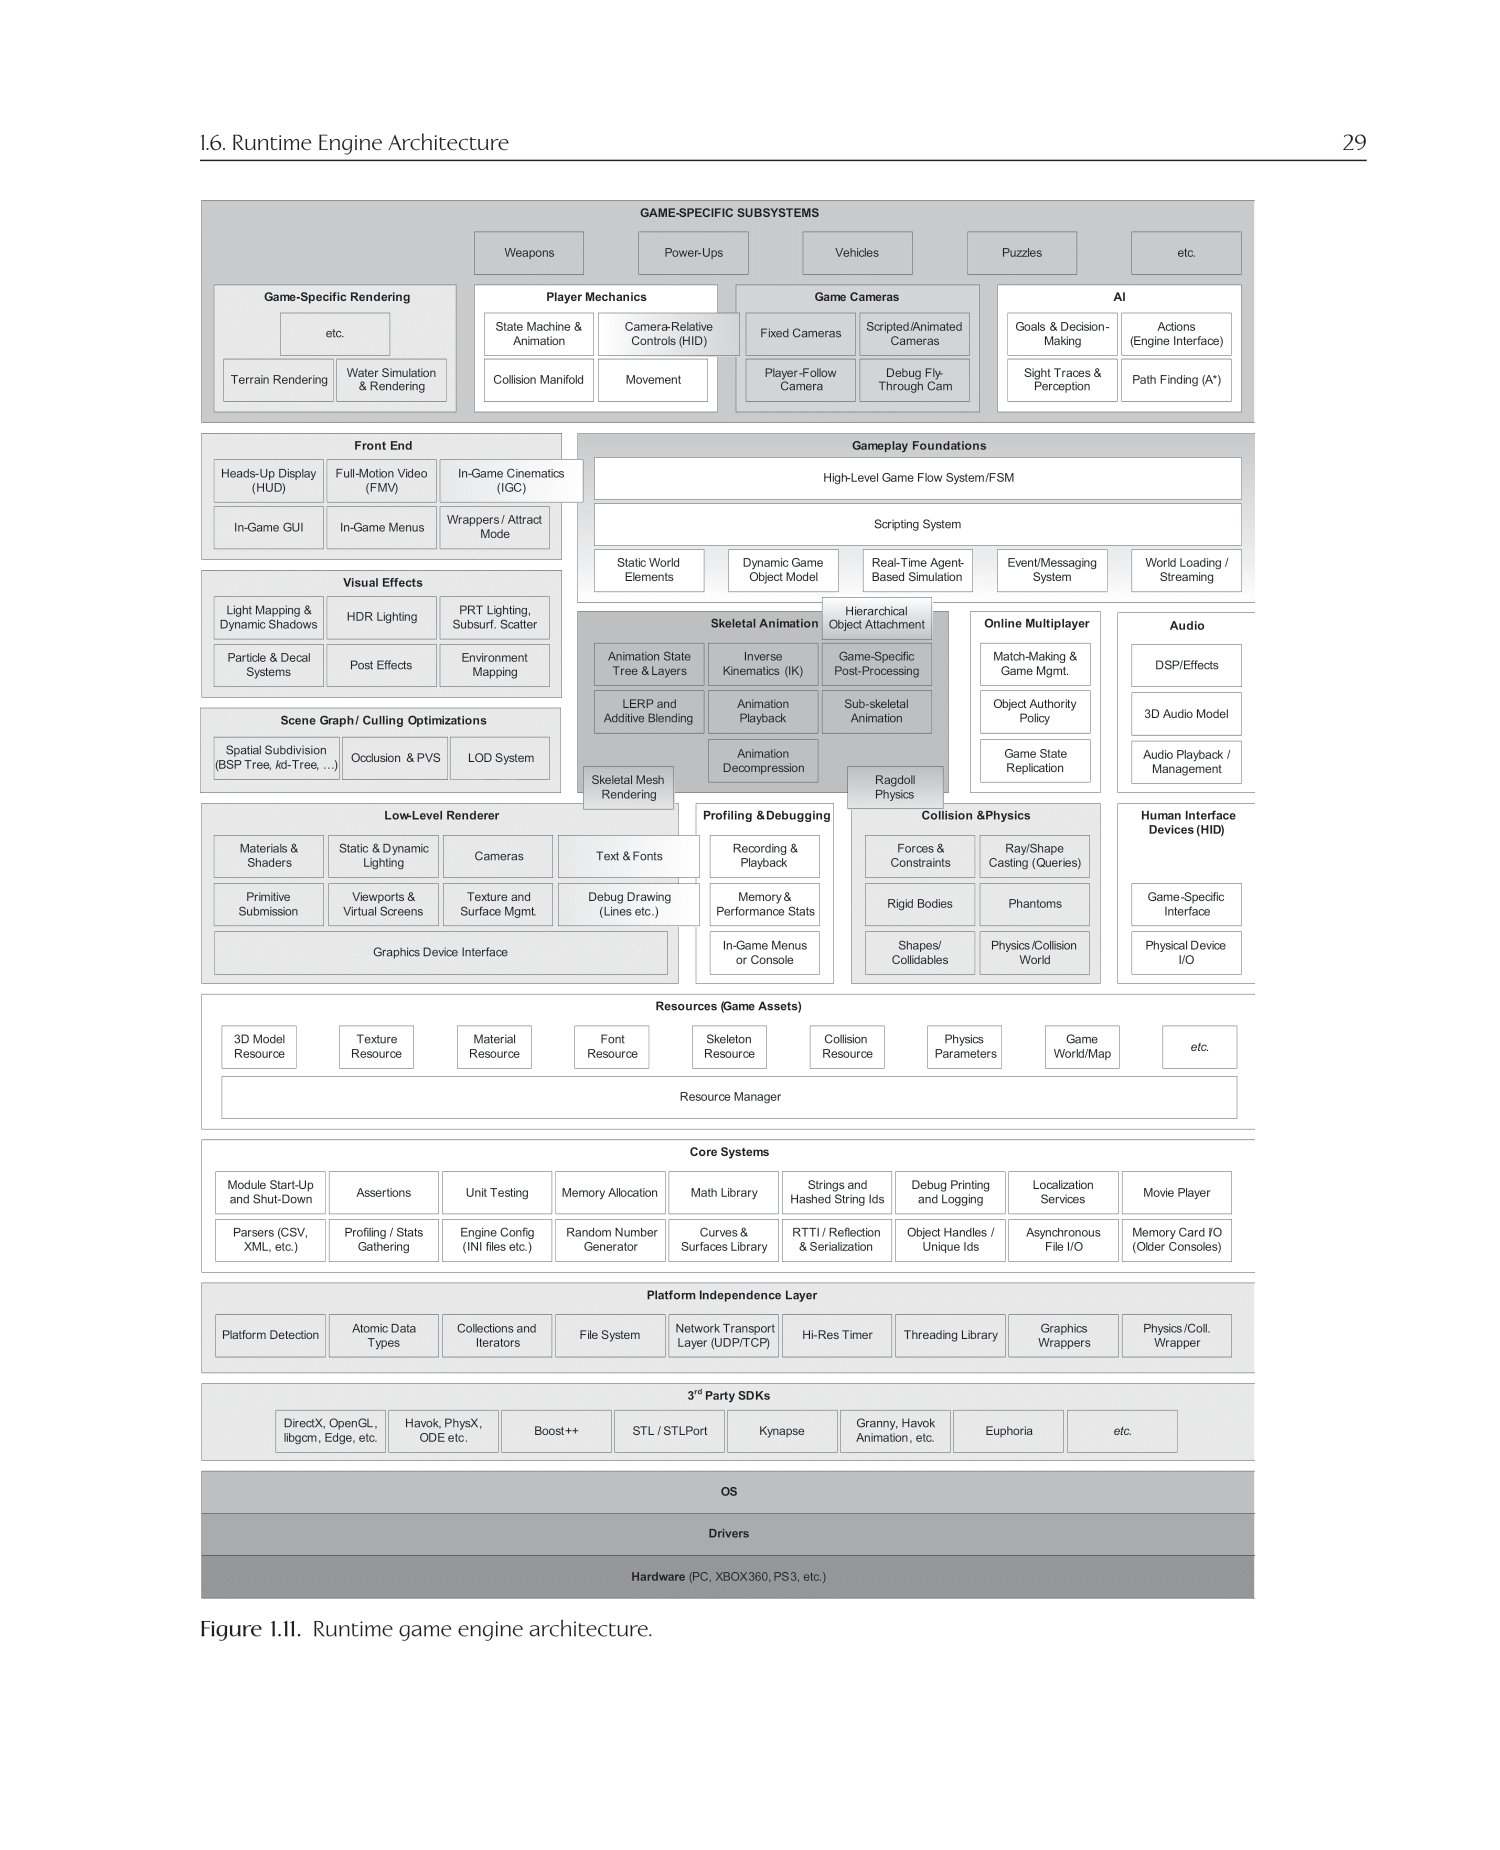
\includegraphics[width=\textwidth]{./resources/engine_arch.png}

\newpage
    % \chapter{系統說明}

\section{使用技術}

\subsection{使用語言}

使用 C++ 11 作為主要開發語言,使用 msys2 作為套件管理器 \footnote{在 Windows 上,沒有套件管理器會非常痛苦} ,CMake 建置專案,
使用 doxygen 工具將註解轉換 documentation, cppcheck C++ 的靜態程式碼分析器

\begin{itemize}
	\item{Slack}
		\subitem{團隊協作軟體,用於溝通紀錄}
	\item{Trello}
		\subitem{看板軟體,用於工作進度管理}
	\item{git, github}
		\subitem{版本控制}
\end{itemize}

TODO 寫多一點

\subsubsection{為何選 C++ 做為開發引擎之語言?}

因為 C++ 讓開發者可以自由掌控記憶體,讓開發者可以精確的控制變數的生命週期,沒有垃圾回收(Garbage Collection),這對於效能注重的遊戲引擎來說相當重要;
比 C 來得高階但效能卻沒損失很多;C++ 歷史悠久且有許多精良的函式庫可以使用。 \cite{WhyCppUsedInGameEngine}

\subsubsection{使用函式庫}

\begin{itemize}
	\item{\href{https://www.sfml-dev.org/}{SFML}}
		\subitem{一個 C++ 的跨平台用於遊戲、多媒體程式開發的函式庫,於此專案中用於 Input 及窗口操作等}

	\item{OpenGL + \href{https://github.com/Dav1dde/glad}{glad}}
		\subitem{一個跨平台的 API ,使用 glad 載入器}

	\item{\href{https://github.com/ocornut/imgui}{imgui}}
		\subitem{一個輕量、快速的 Immediate Mode GUI 函式庫,常在遊戲開發、工具開發等使用,於此專案中用於編輯器的 UI 開發。}

	\item{\href{https://github.com/gabime/spdlog}{spdlog}}
		\subitem{一個輕量、快速的 Logging 函式庫,於此專案中用於處理除錯訊息。}

	\item{\href{https://github.com/mlabbe/nativefiledialog}{nativefiledialog}}
		\subitem{小型的 Open File Dialog 函式庫,於此專案中用於處理開啟檔案視窗。}

	\item{\href{https://github.com/juliettef/IconFontCppHeaders}{IconFontCppHeaders}}
		\subitem{字體的 Helper Headers,於此專案中用於引入自訂字體。}

	\item{\href{https://github.com/fmtlib/fmt}{fmt}}
		\subitem{補足了 C++ 標準庫缺少的格式化輸出輸入。}

	\item{\href{https://github.com/g-truc/glm}{glm}}
		\subitem{OpenGL 數學函式庫,於此專案中用於處理向量、投影等相關數學函式。}

	\item{\href{https://github.com/USCiLab/cereal}{cereal}}
		\subitem{C++ 缺少的序列化函式庫,於此專案中用於序列化儲存資源。}

	\item{\href{https://github.com/google/re2}{re2}}
		\subitem{來自 Google 的 Regular Expression 函式庫,標準庫的有夠慢(確信。}

	\item{\href{}{}}
		\subitem{}
 \end{itemize}

    \chapter{系統實作結果}

\section{引擎介紹}

\subsection{架構}
\label{sub:架構}

\subsubsection{流程圖} % (fold)
\label{ssub:流程圖}



\subsubsection{架構圖} % (fold)
\label{ssub:架構圖}

RishEngine 是由眾多模塊組合而成,就像一個大工具包一樣,給遊戲開發者提供了許多功能:

\begin{itemize}
\item{Core}
    \SubItem{核心模塊,提供了許多基礎功能,例如:檔案系統、視窗、事件、輸出入等功能}
\item{Scene}
    \SubItem{場景模塊,提供了 ECS 和一些跟遊戲物件管理的功能}
\item{Layer}
    \SubItem{提供引擎像是圖層一樣操控遊戲畫面、UI}
\item{Renderer}
    \SubItem{渲染模塊,渲染的基礎建設}
\item{Physics}
    \SubItem{物理引擎,讓東西能動起來}
\item{Particle}
    \SubItem{粒子效果}
\item{Editor}
    \SubItem{編輯器,提供了讓遊戲開發者編輯的工具}
\end{itemize}

\begin{figure}[h]
    \begin{center}
    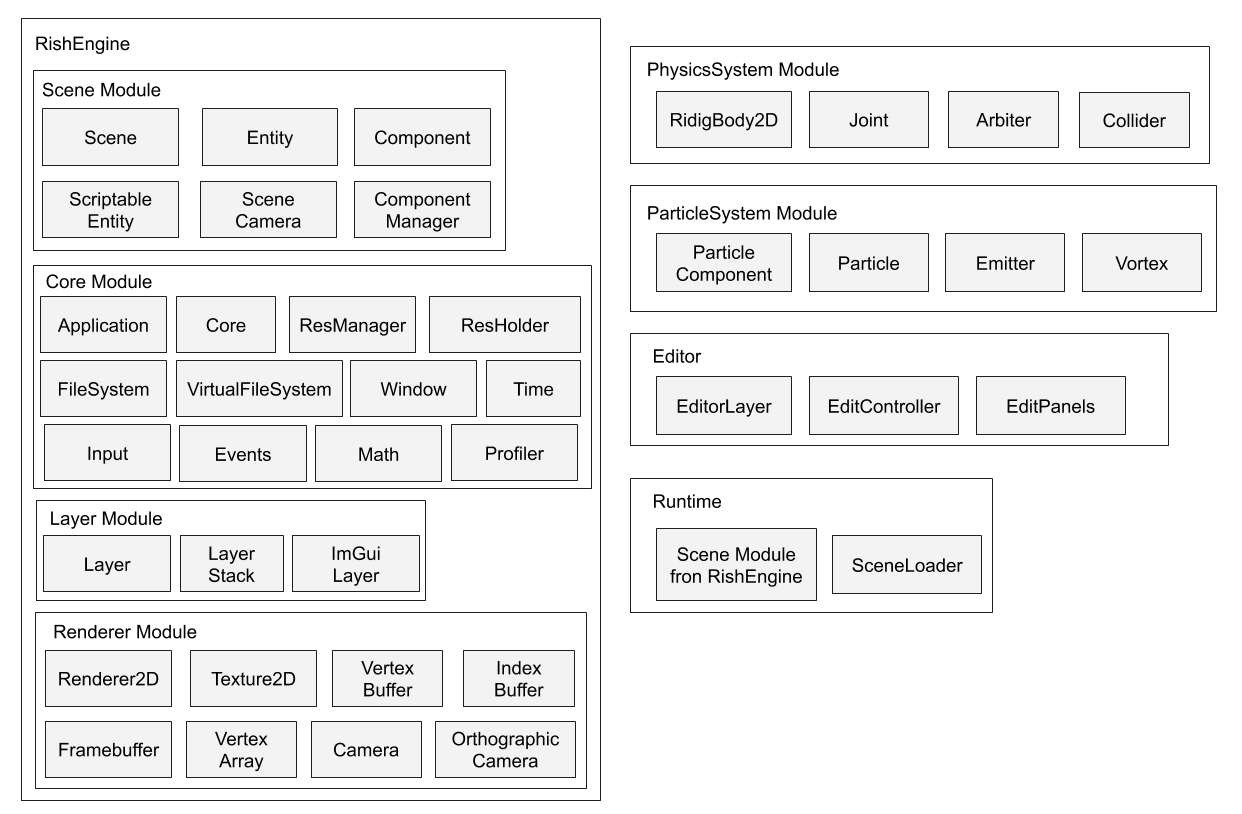
\includegraphics[width=\textwidth]{./resources/RishEngine_arch.png}
    \end{center}
\caption{RishEngine 架構}
\label{fig:RishEngineArch}
\end{figure}


%  Engine
\import{ch4/}{ecs.tex}
\import{ch4/}{batch_rendering.tex}
\import{ch4/}{particle_system.tex}
\import{ch4/}{2d_lighting.tex}
\import{ch4/}{scriptable_entity.tex}
\import{ch4/}{physics.tex}

% Editor
\import{ch4/}{editor.tex}

\newpage
    % \chapter{結論與未來展望}

\newpage
    % \chapter{心得}

\paragraph{Roy} % (fold)
\label{par:Roy}


其實從高中初次接觸程式設計以來,我一直想做的事情便是寫一個自己的遊戲引擎,從高中時初次嘗試撰寫 ADV 類型的遊戲引擎(但受限當時的程式能力,並沒有完成),而到了大學時,我從很早(大概大二)便找好組員,並且也在系上課程的多個專案中不斷地練習和磨合我們之間的合作,我想做的事便是寫一個屬於自己的遊戲引擎。

從三年級下學期開始,經過了九個月的的開發,坐在電腦前數百小時的奮鬥,我們 RISH 終於將 RishEngine 的功能告一個段落,儘管有些功能是因為專案時程以及目前能力而有缺憾,但即便如此我們還是完成了這個專案,我們開發了一款 2D 的遊戲引擎,具有 ECS、有引擎編輯器、有 Batch Rendering、有 2D Lighting、有物理引擎、有 Particle System 等。

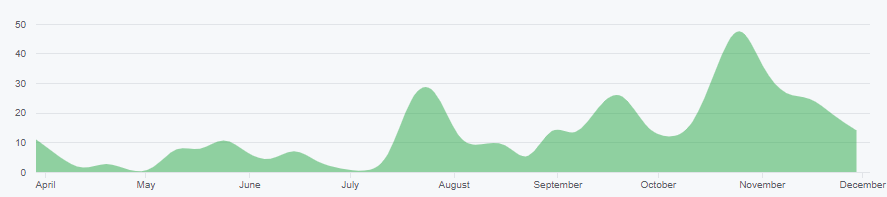
\includegraphics[width=\textwidth]{./resources/commit.png}

而在開發每項功能前,都花了一到兩個星期在做資料搜尋、自學,接著做出最小可行的 Demo,僅僅做出功能還不夠,因為我們做得是遊戲引擎,所以還得將 API 打磨,不斷得去想、擴充功能,因為引擎就是得提供許多功能給遊戲開發者,而在引擎開發階段時,每個功能寫出來之後,還得切換身分到遊戲開發者,試圖用自己做出的引擎來打造遊戲,透過這個過程來除錯和發想可以增加的新功能,一直不斷的迭代,而這個過程是相當漫長和痛苦的,常常在和組員討論時一個功能的規格(spec)時,往往最後都覺得很迷惘,總是覺得這個功能不夠好,但還是得在現實與理想中取捨。

在這次的專案中我也學到了很多東西,像是如何有效與人溝通和合作,表達自己的想法給對方清楚理解,當然過程中勢必有磨合的時期,因為我們是只有四個人的小組,所以作為組長的我理所當然會處理許多工作,也必須擔當起管理的責任,畢竟繁雜的工作量由一個人扛起也過於不切實際,清楚了解到除了程式之外管理和與人相處溝通之道也相當重要。

這個畢業專題算是完成了我其中的一個心願,自幹一個遊戲引擎,也是我目前處理過最多行的程式,算是我的一個小小的里程碑。

% paragraph Roy (end)

\newpage

    \printbibliography

\end{document}
